\documentclass[lang=cn,11pt]{elegantbook}
\usepackage[utf8]{inputenc}
\usepackage[UTF8]{ctex}
\usepackage{amsmath}%
\usepackage{amssymb}%
\usepackage{algorithm}
\usepackage{algorithmic}
\usepackage{graphicx}
\usepackage{pdfpages}
\usepackage{biblatex}      % 用于参考文献管理
\addbibresource{ref.bib}  % 引入 bib 文件

\usepackage{listings}
\usepackage{xcolor}
\lstset{
  language=Matlab,                % 设置代码语言为 MATLAB
  basicstyle=\ttfamily\small,     % 代码的基本字体和大小
  numbers=left,                   % 在代码左侧显示行号
  numberstyle=\tiny,              % 行号的字体大小
  stepnumber=1,                   % 行号递增步长
  numbersep=10pt,                 % 行号与代码间的间隔
  keywordstyle=\color{blue},      % 关键字颜色
  commentstyle=\color{green},     % 注释颜色
  stringstyle=\color{red},        % 字符串颜色
  showstringspaces=false,         % 不显示字符串中的空格
  breaklines=true,                % 自动换行
  frame=single                    % 给代码加一个边框
}


\title{Math 571: Numerical Linear Algebra}
\subtitle{Following Trefethen-Bau's book}

\begin{document}
\frontmatter
\tableofcontents
\mainmatter





\chapter{tensor product and matrix multiplication}
这里我们放弃陈述两个 over 同一 field 的 vector spaces 的 tensor product 的 algebraic definition, 直接看应用的. (完整的 definition 是两个 over 同一个 ring 的 modules $A,B$, 取它们 free abelian group generated by $A\times B$, 再 quotient 掉一个用来形成 bilinearity 的 subgroup, 就是它们的 tensor product. 当这两个东西是 vector spaces 时, 它们并且是 isomorphic to 其对应的 bilinear functional vector space的.)
\begin{definition}{(not rigorous) tensor product}
令 $V,W$ be vector spaces over $\bF$, 我们定义一个 vector 与 vector 之间的 tensor product operation:
$$
\otimes :(v,w) \mapsto v \otimes w
$$
s.t. 对于 $V, W$ 的 basis $e_1, \cdots, e_n$ 和 $\epsilon_1, \epsilon_m$, 我们给每个 $(e_i, \epsilon_j)$ 都赋予一个不同的 image $e_i \otimes \epsilon_j$,  其 over $\bF$ 具有 bilinear 性.\\
对于 
$$
V \otimes W : = span(\{ e_i \otimes e_j \mid 1 \leq i \leq n, 1\leq j\leq m    \})
$$
$V \otimes W $ 也是一个 over $\bF$ 的 vector space, 且 $\dim(V \otimes W) = mn$.
\end{definition}

\begin{proposition}{representing tensor product as matrix}
 如果我们有两个矩阵：
\[
A = \begin{bmatrix} a_{11} & a_{12} \\ a_{21} & a_{22} \end{bmatrix}, \quad
B = \begin{bmatrix} b_{11} & b_{12} \\ b_{21} & b_{22} \end{bmatrix}
\]
可以把它们的 tensor product \( A \otimes B \) 表示为：
\[
A \otimes B =
\begin{bmatrix} 
a_{11} B & a_{12} B \\ 
a_{21} B & a_{22} B 
\end{bmatrix}
=
\begin{bmatrix} 
a_{11} b_{11} & a_{11} b_{12} & a_{12} b_{11} & a_{12} b_{12} \\ 
a_{11} b_{21} & a_{11} b_{22} & a_{12} b_{21} & a_{12} b_{22} \\ 
a_{21} b_{11} & a_{21} b_{12} & a_{22} b_{11} & a_{22} b_{12} \\ 
a_{21} b_{21} & a_{21} b_{22} & a_{22} b_{21} & a_{22} b_{22} 
\end{bmatrix}
\]
can verify: 这个表示是符合 tensor product 的 bilinearity 的.
(我们可以把 $A$, $B$ 分别看作 $m\times n$, $p \times q$ dim 的向量, 这个 $A \otimes B$ 是 $m\times n \times p\times q$ dim 的向量.)
\end{proposition}

\begin{definition}{outer product of two vectors}
    对于 $v \in \bF^n$, $w \in \bF^m$, 我们定义它们的 outer product $v \otimes w$为:
    $$
    v w := v \otimes w^T = \begin{bmatrix} v_{1}  \\ \cdots  \\v_{n} \end{bmatrix} \otimes\begin{bmatrix} w_{1}  & \cdots  &w_{m} \end{bmatrix} = \begin{bmatrix} v_{1}w^T  \\ \cdots  \\v_{n}w^T \end{bmatrix} = \begin{bmatrix} w_{1}v  & \cdots  &w_{m}v \end{bmatrix}
    $$
\end{definition}

\section{matrix product through outer product}

\begin{theorem}{representing matrix multiplication by outer products}
对于 $m\times n$ 的矩阵 $A$ 和 $n \times k$ 的矩阵 $B$, we have:
\begin{equation}
    A B = \sum_{i=1}^n A_{*i} \otimes B _{i*}
\end{equation}
\end{theorem}
\begin{proof}
    In md.
\end{proof}
\begin{remark}
    两个 vectors 的 outer product, 一\textbf{定是一个 rank 为 1 的 matrix}. 因为它每一 column 都是 $v$ 的一个倍数.\\
    但是我们可以累加 $n$ 个这样的 outer products, 从而得到一个可以是 full rank n 的矩阵. (我们知道当然, 矩阵相加不保留 rank.)
\end{remark}


\chapter{orthogonal vectors and matrices}

\begin{definition}{adjoint(hermitian conjugate)}
\[
    ^*:
    A = \begin{bmatrix} a_{11} & a_{12} \\ a_{21} & a_{22}   \\a_{31} & a_{32}  \end{bmatrix}
    \mapsto A^* =  \begin{bmatrix} \overline{a_{11}} & \overline{a_{21}}  &\overline{a_{31}} \\ \overline{a_{12}} & \overline{a_{22}} & \overline{a_{32}}   \end{bmatrix}
    \]
(where each overline means complex conjuate.)
\end{definition}
\begin{remark}
    Can easily comfirm:
    $$
    (AB)^* = B^* A^*
    $$
\end{remark}



\begin{definition}{standard inner product and norm on $\bC^m$}
The \textbf{standard inner product}:
$$
<x,y> := x^* y  = \sum_{i=1}^m \overline{x_i} y_i
$$
The \textbf{standard norm}:
$$
||x|| : =  \sqrt{x^* x}
$$
\end{definition}
\begin{remark}
$$
\sqrt{x^* x} = \sqrt{\sum_{i=1}^m |x_i|^2}
$$, 其中 $|x_i| = |a+ bi| = \sqrt{a^2 + b^2}$, \\
\textbf{Note: It is actually $\sqrt{\overline{x_i} x_i}$, but not $\sqrt{x_i^2}$, 这是因为 $\sqrt{\overline{x_i} x_i}$ 等于这个 complex scalar isomorphic 到 $\bR^2$ 上的 Euclidean norm,}\\ 
这是因为两个复数相乘等于长度相乘幅角相加, 而 conjugate 的幅角是相反的, \textbf{所以 conjugate 之间相乘等于幅角相互抵消, 结果在 positive real axis 上, 取开方得到长度.} \\
而平方得到的则是一个转两次的幅角.
\end{remark}
\begin{remark}
    Can easily verifies:
    $$
    <a,b>_{\bC} = \overline{<b,a>_{\bC}}
    $$
    且注意: By bilinearity, \textbf{对于 $a$ 上的 scaling 在拿出 inner product 外后要进行 conjugate.}
\end{remark}

\begin{definition}{orthogonal, orthonomal vectors}
    Say $x, y \in \bC^m$ 是 orthogonal vectors, if $x^* y = 0$.\\
    Say $S \sub \bC^m$ 是 orthogonal 的, 如果其中的 vectors 相互 orthogonal.\\
    Say $S \sub \bC^m$ 是 orthonomal 的, 如果其中的 vectors 相互 orthogonal, 并且每个 vector 的 norm 都是 1.
\end{definition}

\begin{theorem}{orthogonal $\implies$ lin.ind}
    orthogonal 的 vectors 一定 linearly independent.
\end{theorem}
\begin{proof}
    trivial.
\end{proof}
\begin{corollary}
    orthogonal 的 $\dim(V)$ 个 vectors 一定是 $V$ 的一个 basis.
\end{corollary}


\section{decomposing vector by an orthonormal set}
\begin{theorem}{decomposing vector by an orthonormal set}
给定 $\bC^m$ 中的一个 orthonormal set $\{q_1, \cdots, q_n\}$ (by inner product $<\cdot>$, 这里以 standard complex inner product 为例), 
\\对于一个 arbitrary vector $v$, 我们 define:
$$
r:= v - \sum_{i=1}^n <q_i, v>   q_i
$$
Claim: 这个 \textbf{$r$ is orthogonal to $\{q_1, \cdots, q_n\}$,} 即我们把这个 $v$ 分解成了在这个 orthonormal set 上的投影与一个和它们都正交的 vector.
\end{theorem}
\begin{proof}
    注意: 由于 $q_i$ 都是 unit vectors, $$<q_i, v> q_i = \frac{v}{||v||} \cos \alpha = proj_{q_i}(v)$$\textbf{ is the projection of $v$ onto the direction of $q_i$.}\\
我们在两边取和 $q_i$ 的 inner product, for each $i$. 由 linearity 可拆开, 由 orthgonality 可得到:
$$
<q_i,r> = <q_i,v> - <q_i,v><q_i,q_i>
$$
并且由于 $q_i$ 是 unit vector, 得到 $<q_i,q_i>=1$, 从而右边为 0.
\end{proof}
\begin{remark}
    如果 $n=m$, 那么 $r=0$, 我们把 arbitrary vector 分解成了 $\{q_1, \cdots, q_n\}$ 方向上的向量, 相当于对它进行了 change of basis. 这个 change of basis matrix 就等于 $\begin{bmatrix} q_1  & \cdots  & q_n \end{bmatrix}^T$.
\end{remark}


 对于 unit vector $w$, 我们刚才已经展示了一个 arbitrary vector $v$ 在它上面的 projection 是:$$proj_w (v) = <w, v> w  $$
 现在我们引入另一个形式的 projection 表达: projection matrix

\begin{theorem}{projection matrix}
对于任意的 \textbf{unit vector $w$}, we have
$$proj_w (v) = (w \otimes w^*) v $$
其中 $w\otimes w^*$ is called the \textbf{projection matrix} onto $w$.
\end{theorem}
\begin{proof}
    In md.
\textbf{    Notice that this matrix is rank 1.}
\end{proof}


\begin{definition}{unitrary matrix}
一个 square matrix $Q \in \bC^{m\times m}$ 被称为 unitrary 的, if $Q^* = Q^{-1}$.
\end{definition}

\begin{remark}
    unitrary: 即 $QQ^* = Q^*Q = I$. \\
    \textbf{In real case, 它被称为 orthogonal matrix.}
\end{remark}


\begin{theorem}{unitrary matrix 的充要条件}
$Q \in \bC^{m\times m}$ is unitrary $\Longleftrightarrow $ \textbf{its columns are orthonormal} $\Longleftrightarrow$ \textbf{its rows are orthonormal} 
\end{theorem}
\begin{proof}
    显然, 因为 unitrary $\Longleftrightarrow QQ^* = Q^*Q = I$ $\Longleftrightarrow  <q_i, q_j> = \delta_{ij}$
\end{proof}



\begin{theorem}{unitrary transfromation preserves inner product and length}
如果 $Q \in \bC^{m\times m}$ is unitrary, 那么对于任意的 $x,y \in \bC^m$, 都有:
$$
(Qx)^* (Qy) = x^*y
$$
并且自然得到 $$||Qx|| = ||x||
$$
\end{theorem}
\begin{proof}
Follows from: $(AB)^*= B^* A^*$:  $$(Qx)^* (Qy) = x^*Q^*Qy= x^*y
$$
\end{proof}
\begin{remark}
    并不 preserve 自定义的 inner product, 只 \textbf{preserve standard inner product 和 standard norm.}
\end{remark}



\chapter{norms}

\begin{definition}{norm}
一个 norm on a vector space $V$是一个满足:
\begin{enumerate}
    \item nonnegativity (0 iff $x=0$)
    \item trianglar ineq
    \item homogenity
\end{enumerate}
的 function $||\cdot||:V \rar \bR$
\end{definition}


\section{norms on $\bC^m$}
\begin{example}
以下为 $\bC^m$ 上的典型 norms: (absolute value 表示 length, 即 $\sqrt{x^*x}$) \\
$Lp$-norm: $p$ 越大, the largest length dimension 占 norm 的比重就越大
$$
    ||x||_p = (\sum_{i=1}^m |x_i|^p)^{\frac{1}{p}}
$$
\textbf{$L_\infty$-norm:最长维度.}$$
    ||x||_\infty = \max_i |x_i|
    $$
weighted norm: 给定一个 norm $||\cdot||_k$, 这是 weighted version of this norm. 其中 \textbf{$W$ 是一个 diagonal matrix, diag 上的是 weights.}
$$
||x||_{W,k}= ||Wx||_{k}
$$
\pic[0.5]{01-fundamentals.assets/Screenshot 2025-01-29 at 22.41.10.png}
\pic[0.4]{01-fundamentals.assets/Screenshot 2025-01-29 at 22.41.52.png}
\end{example}





\section{operator norms on matrix spaces}

We know: 所有的 $m \times n$ matrix, every entry in $\bF$ 也是一个 vector space of $\dim nm$ over $\bF$.\\
所以我们当然也可以给 matrix 赋范.\\
matrix 代表一个 linear transformation, 所以 norm 的意义实际上是它 stretch vector 的程度的一种评估.

\begin{example}
\begin{definition}{operator norm}
 $$
||A||_{(m,n)} = \sup _{z\in \bC^m, ||z||_n = 1  } ||Ax||_m
$$
induced by vector norm. 表示它\textbf{ stretch vector 的最大程度}. 其中, source 和 image vector 分别用 norm n,m 来判定.\\
如果 source 和 image vector 的 norm 是一样的, 比如都使用某个 $L_p$ norm, 那么我们可以用单个符号表示(induced by $p$-norm):$$ ||A||_{p} = \sup _{z\in \bC^m, ||z||_p= 1  } ||Ax||_p
$$
(这更加常用, 因为通常我们会对 source 和 image vector 的大小使用相同的评估)
\end{definition}

\begin{proposition}{\textbf{diagonal matrix 的 norm: reduced to max diag element}}
    如果 $D$ 是一个 diagonal matrix, 那么不论取什么 $p$-norm, 我们都有: $$
    ||D||_p = \max_{1 \leq i \leq m} |d_i|
    $$
    其中 $d_i$ 为对角线上的元素.
\end{proposition}
\begin{proof}
很直观. 我们要把一个以 $||\cdot||_p$ 为衡量的 unit ball 上的哪个 vector 被拉伸的程度最大,  而 diagonal matrix 把每个坐标 $i$ 上的点固定放大 $d_i$ 倍, \\
因而选择绝对值最大的 $d_k$, 拉伸最大的 vector 一定是 $[0\cdots1\cdots0]$ where only the $k$-th coordinate is $1$, 因为这个 ball 上所有的 vectors 原本的 norm 都是一样的, 而这个 vector 完整地吃到了最大的拉伸程度, 其他 vectors 都或多或少吃到了其他 $d_i$ 的拉伸效果.
\end{proof}

\begin{proposition}{\textbf{1-norm: reduced to max column sum}}
\begin{equation}
    ||A||_1 =  \max_{1 \leq j \leq n}  ||A_{*j}||_1
\end{equation}
\textbf{matrix 的 1-norm 实则就是 1-norm 最大列的 1-norm.}
\end{proposition}
\begin{proof}
    因为 
    $$
    ||Ax||_1 = || \sum_i x_j a_j ||_1 \leq \sum_j |x_j| |a_j||_1
    $$
    并且 $\sum_j |x_j| = 1$, 因而这个和 $\leq \max_j ||a_j||_1$.\\
    并且我们发现, 这个值是可以取到的: suppose $||a_k||_1$ 最大, 那么取 $e_k$ 就可以了.\\
直观而言, 由于 1-norm 的单位球和它的 image 都是一个多面体, 它取到最大的点一定是某个顶点. 以这里的 $\bR^2$ 为例, 一定是 $e_1$, $e_2$ 中的一个.
\end{proof}

\begin{proposition}{\textbf{$\infty$-norm: reduced to max row sum}}
    \begin{equation}
    ||A||_1 =  \max_{1 \leq i \leq m}  ||A_{i*}||_1
\end{equation}
\textbf{matrix 的 $\infty$-norm 实则就是 $1$-norm 最大行的 $1$-norm}.\\
\end{proposition}
\begin{proof}
直观上, image 的 sup norm 只取最大的那一个 entry，因而一定是取矩阵\textbf{总(absolute)长度最大的一列, 因为每一列都只贡献 image vector 中的一个 entry. }
并且, 我们注意到, source vector (on单位球) 包括了\textbf{所有的最大 entry 为 $1$ 的 vectors}，这些 vectors 的 sup norm 都是一样的。而要使得 image vector 的 entries 尽可能大, 我们一定会\textbf{取所有 entries 都为 1 的 vector 作为 input.}
\pic[0.5]{01-fundamentals.assets/image-20250130003611232.png}
Note: sup norm 的单位球和它的 image 也都是一个多面体.

\end{proof}

\end{example}




\section{Caychy-Swartz and Frobeniu norm}

\begin{theorem}{Hölder inequility and Cachy-Swartz}
Let $x,y \in \bC^m$, let $p\geq 1, q \leq \infty$ s.t. 
$$
\frac{1}{p} + \frac{1}{q} = 1
$$
\textbf{Holder ineq:}
\begin{equation}
    |x^*y| \leq ||x||_p ||y||_q
\end{equation}
\textbf{Cauchy-Schwarz ineq(special case of Hölder ineq when $p=q=2$)}:
\begin{equation}
    |x^*y| \leq ||x||_2 ||y||_2
\end{equation}

\end{theorem}
\begin{remark}
    Holder' ineq 可以 generalize 到 $L_p$-measurable space, Cauchy-Swartz 可以推广到任何 Banach space. 此处不展开.
\end{remark}
\begin{proof}
 \textbf{of Cauchy-Swartz:  } \\
 By homogenity of inner product and norm, it \textbf{suffices to prove for unit vector $u,v$.}\\
 $$(u-v)^2 = ||u||^2 -2u^* v + ||v||^2 $$
 因而
 $$
 u^*v \leq \frac{||u||^2 + ||v||^2}{2} = 1 = ||u|| \, ||v||
 $$
 等号成立 iff $u =v$.
\end{proof}


\begin{example}
    Applying Cauchy-Swartz 可以发现: row vector 的 matrix 2-norm 等于它 (adjointed) 作为 vector 的 vector 2-norm.\\
    这是因为 consider $a := A^*$, 则 
    $||Ax|| = |a^* x| \leq ||a||_2 ||x||_2$, 因而总有 $||Ax|| / ||x||_2 \leq ||a||_2$. 并且这个等号可以取到, by taking $x := a$.
\end{example}



\begin{example}

    任取两个 vectors $u,v$, 它们 outer product 成的 rank-one matrix, 其 operator 2-norm 小于等于它们自身的 2-norm 的乘积.\\
    $$
    ||Ax||_2  = ||uv^* x||_2 = ||u||_2 |v^*x| \leq ||u||_2 ||v||_2 ||x||_2
    $$
    这是因为: $u  v^*$ 这一 outer product 乘以一个向量, 即每行都是 $v^*$ 的一个倍数 ($u_i$ 倍) 的矩阵乘以这个向量. 因而, 每行得到的都是 $u_i$ 乘上 $v^* x$ 这个 inner product, 最后得到的就是
    $$
    Ax = (v^*x) u
    $$
    即 $u$ 的一个倍数, 这个倍数等于 $v^* x$. 
\end{example}


\begin{example}
\begin{theorem}
\begin{equation}
    ||AB||_{(l,n)} \leq ||A||_{(l,m)} ||B||_{(m,n)}
\end{equation}
\end{theorem}
(并且通常取不到等号.)
\begin{proof}
    不证明了. Playing with definition 加上 Cauchy-Swartz.
\end{proof}
\end{example}


\begin{definition}{Frobenious norm}
    $$
    ||A||_F := (\sum_m \sum_n |a_{ij}|^2)
    $$
    等于把这个 matrix 展开为 $m\times n$ 的 vector 的 vector 2-norm.
\end{definition}


\begin{theorem}{equivalent form of Frobenius norm}
    \begin{equation}
        ||A||_F = \sqrt{tr(A^*A)} = \sqrt{tr(AA^*)}
    \end{equation}
\end{theorem}
\begin{proof}
    trivial. $A^*A$, $AA^*$ 的 trace 上每个元素, 都是 $A$ 的一行与自己的 dot product, 即这一行作为 row vector 的 2-norm 的平方; 
\end{proof}

\begin{proposition}
    \begin{equation}
        ||AB||^2_F \leq ||A||^2_F ||B||^2_F
    \end{equation}
\end{proposition}
\begin{proof}
    因为 $AB$ 的每个 entry $c_{ij}$ 作为 $A_i$ 和 $B_j$ 的 inner product, by Cauchy-Swartz, have 
    $$
    |c_{ij}| \leq ||A_i||_2 ||B_i||_2
    $$
因而:
\begin{align}
    ||AB||_F  &\leq \sum_n \sum_m (||A_i||_2 |||B_j||_2) \\ 
    & = (\sum_n ||A_i||_2)(\sum_m ||B_j||_2) \\
    & = ||A||_F ||B||_F
\end{align}
(虽然这看起来很不对, 但容易验证, 这上下两个 sum 是相等的. )
\end{proof}

\begin{theorem}{unitrary matrix preserves 2-norm 和 Frobenius norm}
    Let $Q $ be unitrary, then
    $$
    ||QA||_2 = ||A||_2, ||QA||_F = ||A||_F
    $$
\end{theorem}
\begin{proof}
    因为 $||Qx||_2 = ||x||_2$ for each $x$. \\
    Frobenius norm: 
    $$
    tr((UA)^*(UA) ) = tr(A^*U^*UA) = tr(A^*A) 
    $$
\end{proof}







\chapter{SVD}
SVD 的 motivation: 一个 linear transformation 可以通过 \textbf{unit sphere 的 image 来唯一确定}. 并且, 这个 \textbf{unit sphere 的 image 一定是一个 hyperellipse (高维椭圆).}

\begin{definition}{principal semiaxes, singular value}
对于一个 linear transformation $T: \bR^n \rar \bR^m$, 我们 denote the unit sphere in $\bR^n$ as $S$, 把 $T(S)$ 这一 hyperellipse 中相互 orthogonal 的各轴上的 vectors 表示为 $\{  \sigma_1 u_1, \cdots, \sigma_nu_n    \}$. 其中 $\sigma_i$ decsending, $u_1,\cdots,u_n$ 为 unit vectors. \\
我们称 $u_1,\cdots,u_n$  为 left singular vectors, $\sigma_1, \cdots, \sigma_n$ 为 singular values, 而 $\{v_1,\cdots,v_m\}$ 作为
    
\end{definition}


\section{reduced SVD}













\chapter{QR factorization}

\section{projector}

\begin{definition}
    我们称一个 operator $P: \mathbb{C}^n \rightarrow \mathbb{C}^n$ 为一个 projector, if \[
    P^2  = P
    \]
Note: \textbf{不要求是 linear 的.} For linear case, 这是一个\textbf{ idempotent linear map.}
(而我们将主要关注于 linear orthogonal projector.)
\end{definition}
\begin{remark}
一个 projector 总有: \[
P^m = P
\]
对于任意 $m$ 次 composition.\\
即: 在第一次作用后, 之后再对其结果进行这一映射不作出任何改变. \\
直观: 这个映射的效果是把一个向量投影到一个低维度子空间上, 从而, 在作用过一次后, 再次施加这一映射将没有任何改变.\\


\end{remark}

\begin{remark}
    对于 orthogonal 的 projector, 我们称其为 orthogonal projector; 对于 non-orthogonal 的 projector, 我们称其为 oblique projector.\\
    
\end{remark}


\begin{remark}
    projector 虽然不保证是 linear 的, 但是要么是 linear 的, 要么就是个 affine transformation. 和 linear 也差不多. 不用在意这些细节. 
\end{remark}

以下, 我们都只考虑 projector linear 的情况. nonlinear 的情况是类似的.

\begin{lemma}
我们发现, 一个 projector $P$ 沿着 $S_1 := \ker(P)$ 把空间投影到 $S_2 :=im(P)$ 上.
\end{lemma}

\begin{lemma}
    一个 projector 的 eigenvalue 只有可能是 $0$ 或者 $1$. 它的 SVD 同时也是 eigenvalue decomposition: \[
    P = Q \Sigma Q^*
    \]
    其中 $\Sigma$ 是一个前面全 1, 后面全 0 的对角矩阵.
\end{lemma}


\begin{lemma}{complement projector}
    如果 $P$ 是一个 projector, 那么 $I-P$ 也是一个 projector.\\
    我们称 $I-P$ 为 $P$ 的 complementary projector.\\
    并且我们有: \textbf{complementary projector 的 ker 是原 projector 的 im, im 是原 projector 的 ker.}
\end{lemma}

\begin{remark}
    $P$ 把 vectors 沿着 $S_1$ 投影到 $S_2$; \\
    $I - P$ 把 vectors 沿着 $S_2$ 投影到 $S_1$.
\end{remark}


\begin{definition}{orthogonal projector}
    我们称一个 projector 是 orthogonal projector, 如果 $\ker(P) \bot im(P)$.
\end{definition}

\begin{theorem}
    一个 projector $P$ 是 orthogonal projector $\Longleftrightarrow$ $P = P^*$, 即 $P$ 是 Hermitian 的.
\end{theorem}

\begin{theorem}
    一个 projector $P$ 是 orthogonal projector, 则它的 \textbf{complementary projector $I-P$ 也是 orthogonal projector.}
\end{theorem}

\begin{corollary}
    orthogonal projector $P$ 的 complementary $I-P$ 把 vectors 投影到 $im(P)^{\bot}$ 上. 
\end{corollary}

\section{classical Gram-Schmidt orthogonalization}
classical Gram-Schmidt 是计算 reduced QR 分解的算法.
\begin{figure}
    \centering
    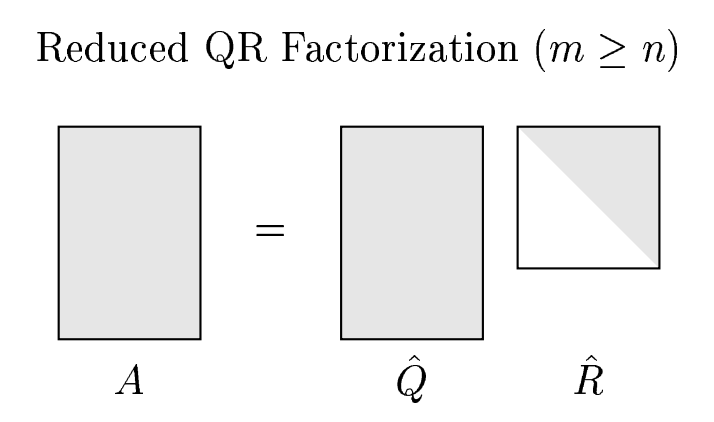
\includegraphics[width=0.5\linewidth]{assets/Screenshot 2025-04-17 at 11.44.46.png}
    \caption{reduced QR}
    \label{fig:reduced QR}
\end{figure}
\subsection{idea of triangular orthogonalization}
classical Gram-Schmidt orthogonalization 的 idea 是: 我们逐列地将 $A$ 的 columns 转变为相互 orthogonal 的新列.\\
具体: 我们每次都把 $a_j$ 减去 $a_1,\cdots, a_{j-1}$ 的 span 包含的成分, 从而制作成和  $a_1,\cdots, a_{j-1}$ 的 span 正交的新列 $q_j$: 
\begin{align*}
q_j := \text{normalized} (& \,a_j - \text{proj}_ {\langle a_1,\cdots,a_{j-1} \rangle} a_j) \\
=  \text{normalized} (& \,a_j- \text{proj}_ {\langle q_1,\cdots,q_{j-1} \rangle} a_j)
\end{align*}
展开这个定义: 
\begin{align*}
v_j&:=a_j-\left(q_1^* a_j\right) q_1-\left(q_2^* a_j\right) q_2-\cdots-\left(q_{j-1}^* a_j\right) q_{j-1}\\
    q_j  &:= v_j / |v_j|  
\end{align*}
这个过程可以通过定义: 
$$
r_{i j}=q_i^* a_j \;(i \neq j), \quad   \left|r_{j j}\right|=\left\|a_j-\sum_{i=1}^{j-1} r_{i j} q_i\right\|_2
$$
(Note that the sign of $r_{j j}$ is not determined. Arbitrarily, we may choose $r_{j j}>0$, in which case we shall finish with a factorization $A=\hat{Q} \hat{R}$ in which $\hat{R}$ has positive entries along the diagonal.)\\
从而这个过程写作: 
\begin{align*}
v_j &:=a_j -  \sum_{i=1}^{j-1} r_{i j} q_i    \\
q_j  &:= v_j / r_{jj}  
\end{align*}
我们发现:
$$
\begin{aligned}
q_1 & =\frac{a_1}{r_{11}} \\
q_2 & =\frac{a_2-r_{12} q_1}{r_{22}}, \\
q_3 & =\frac{a_3-r_{13} q_1-r_{23} q_2}{r_{33}}, \\
& \vdots \\
q_n & =\frac{a_n-\sum_{i=1}^{n-1} r_{i n} q_i}{r_{n n}}
\end{aligned}
$$
这个过程使得: 
\[
a_j = \sum_{i=1}^j r_{ij} q_i
\]从而:
\[
A  = \hat{Q} \hat{R}
\]

\subsection{algorithm}


\begin{algorithm}
\caption{Classical Gram-Schmidt (unstable)}
\begin{algorithmic}[1]
\FOR{$j = 1$ \TO $n$}
    \STATE $v_j \gets a_j$
    \FOR{$i = 1$ \TO $j-1$}
        \STATE $r_{ij} \gets q_i^* a_j$
        \STATE $v_j \gets v_j - r_{ij} q_i$
    \ENDFOR
    \STATE $r_{jj} \gets \|v_j\|_2$
    \STATE $q_j \gets v_j / r_{jj}$
\ENDFOR
\end{algorithmic}
\end{algorithm}




\section{modified Gram-Shimitdt (triangular orthogonalization)}





\section{Household Triangularization}






\chapter{Discrete Fourier transform and FFT algorithms}









\chapter{conditioning and stability\cite{doi:10.1137/1.9780898719574.ch3}}
接下来 chapter 中我们将讨论 numerical analysis 中的两个 fundamental issues: Conditioning 和 Stability. Conditioning 指的是 \textbf{perturbation behavior of a mathematical problem}; 而 Stability 指的是解决这一问题的 \textbf{algorithm 的 perturbation behavior.}

\begin{definition}{problem, problem instance}
我们把一个 problem 看作是一个 function, 把 normed VS $X$ of data map to normed VS $Y$ of solutions. 即: \[
f: X \to Y
\]    
其中, 这个 problem $f$ together with a data point $x$ 被称为一个 \textbf{problem instance}. (比如:输入是 $x$, 问题是求 $x$ 的平方根, $f: x\mapsto \sqrt{x}$, 那么 $f$ together with input $x=3$ 就是一个 problem instance.)
\end{definition}

Conditioning 研究的就是一个 problem instance $(f,x)$, 其附近 solutions 的变动行为.\\
一个 well-conditioned problem instance 就是指, $x$ 附近的 small perturbations 只 lead to small changes; 而 ill-conditioned problem instance 就是指, $x$ 附近的 small perturbations 可能引起 big changes. 


\section{absolute/relative condition number of a problem}
\begin{definition}{absolute condition number}
$\delta x$ 表示 $x$ 附近的一个 small perturbation, 并用 \[
\delta f = f(x + \delta x) - f(x)
\]
来表示 $f$ 随之产生的变化. \\
定义 absolute condition number 为: \[
\hat \kappa(x) := \lim_{\delta \to 0} \sup_{||\delta x || \leq \delta} \frac{ ||\delta f ||_y}{||\delta x||_x}
\]
\end{definition}
\begin{remark}
    即, $x$ 附近比较小的区域上, $f$ 的值随 $x$ 的变化的变化量.\\
   我们发现, 这和导数的定义很相近, 就是加了一个 norm. 当然, 并不完全是. 因为这里取的是 $\sup$. 导数未必存在, 但是这个 $\sup$ 总是存在的(如果 count into infty 的话). absolute condition number 是一种上极限概念, 表示 $x$ 周围的 $f$ 变动幅度最大的值; 而它也不完全是导数值 (recall: 导数是 best linear approximation of this function near this point, 和原 function 的形状是一样的, 这里 take 的是导数的某个 matrix operator norm, determined by 我们对 $y,x$ 使用的 norm)\\
具体: 我们发现, 当 $\delta$ 足够小的时候, we have: $$
\delta f \approx J(x) \delta x
$$
(这里使用 approx, 但是可以严格证明.) 从而, 如果 $f$ differentiable,\[
\hat \kappa(x) := \lim_{\delta \to 0} \sup_{||\delta x || \leq \delta} \frac{ ||J(x) \delta x ||_y}{||\delta x||_x} = ||J(x)||_{x\to y}
\]
简写: \[
    \hat\kappa(x) = ||J(x)||
    \]
\end{remark}


这里还有另外一个 condition number:
\begin{definition}{relative condition number}
\[
\kappa (x) : = \lim_{\delta \to 0} \sup_{||\delta x || \leq \delta}   \bigg(  \frac{||\delta f ||}{||f(x)||} \bigg/   \frac{||\delta x||}{||x||} \bigg)
\]
(recall: $\delta f$ 并不是 $f$ 的倍数而是: \[
\delta f = f(x + \delta x) - f(x)
\]
即 $x$ perturbated 后的函数值和原先的函数值的差.)
\end{definition}
\begin{remark}
    它表示的是, 对于 $x$ 附近的 perturbation, \textbf{$x$ 相对自身的比例变化, 引发的 $f$ 相对自身的比例变化, 的最坏情况.}\\
    对于 differentiable $f$, 有 \[
    \kappa (x) = \frac{||J(x)||_{x\to y}}{||f(x)||_y / ||x||_x}
    \]
\end{remark}

这里对于 absolute/relative condition number 有一种不严谨的记法: 我们把 $\delta x,\delta f$ 看作 infinitesimal (当然,严格的分析里并不存在) 那么可以简写为: 
$$
\hat{\kappa}=\sup _{\delta x} \frac{\|\delta f\|}{\|\delta x\|},\quad  \kappa=\sup _{\delta x}\left(\frac{\|\delta f\|}{\|f(x)\|} / \frac{\|\delta x\|}{\|x\|}\right)
$$

\begin{example}
问题 1.  $f: x\mapsto \frac{x}{2}$, 即把一个数取半. 那么对于任意 $x$ 都有: \[
    \kappa(x) = \frac{||J(x)||}{||f(x)|| / ||x||} = \frac{1/2}{(x/2) / x} = 1
    \]
well-conditioned.\\
问题 2. $f: x\mapsto \sqrt{x}$, 即取一个数的 sqrt, $x>0$, 有: \[
\kappa (x)  =  \frac{||J(x)||}{||f(x)|| / ||x||} =  \frac{1/2\sqrt{x}}{\sqrt{x} / x} = \frac{1}{2}
\]well-conditioned.
\begin{center}
        
\includegraphics[width=0.3\textwidth]{notes/assets/condition1.png} 
        
    \end{center}
\end{example}

\subsection{examples: 两数相减}
\begin{example}
    问题 3: $f: (x_1, x_2)\mapsto x_1 - x_2$ 两数字相减. \[
J(x) = [\frac{\partial f}{\partial x_1}, \frac{\partial f}{\partial x_2}] = [1,-1]
\]
For simplicity, 取 $\infty$-norm, 得到 $||J(x)|| = 2$, 于是 \[
\kappa(x) = \frac{ 2}{|x_1 - x_2| / \max \{ |x_1|, |x_2|\}}
\]
如果 $|x_1 - x_2|$ large 时, $\kappa$ 就会变的很大. 因而 \textbf{this problem is ill-conditioned when $x_1 \approx x_2$.} 这符合 "cancellation error": \textbf{相近的两个数相减会损失有效数字, 放大误差.}\\
For example: 
$$
a=123456.789012, \quad b=123456.789011
$$
它们的差:  $$
a-b=0.000001
$$
如果浮点数只能保留 7 位有效数字 (单精度), 那么 $a$ 被存为 123456.8, $b$ 被存为 123456.8, 相减后结果是 $0.0$ , 完全错误. 这就是 cancellation error：由于精度丢失导致的小差值计算结果失真.
\end{example}

\subsection{example: polynomial 求根}

\begin{example}
    问题 4: polynomial 求根. $f:\mathbb{C}^n \to \mathbb{C}^n$, 把 $n$ 个系数 maps to $n$ 个 roots.\\
我们考虑  $$
p(x)=a_0+a_1 x+a_2 x^2+\cdots+a_n x^n=\sum_{k=0}^n a_k x^k
$$如果 coefficient $a_i$ 被 perturbed by an infinitesimal quantity $\delta a_i$, 那么 the perturbation of root $x_j$ 是多少? 答案是: \[
\delta x_j= -\left(\delta a_i\right) x_j^i / p^{\prime}\left(x_j\right) \label{perturbation of a root given perturbation of a coeff}
\] 
从而对于这个问题:
$$
\kappa_j(a_i)=\frac{\left|\delta x_j\right|}{\left|x_j\right|} \bigg/ \frac{\left|\delta a_i\right|}{\left|a_i\right|}=\frac{\left|a_i x_j^{i-1}\right|}{\left|p^{\prime}\left(x_j\right)\right|}
$$
证明 \ref{perturbation of a root given perturbation of a coeff}:  (非 rigorous)\\
 perturbed polynomial 即: $$
\tilde{p}(x)=p(x)+\delta a_i x^i
$$
我们要求的 perturbation $\delta x_j$,  无法直接得到等式关系. 但是我们知道新的 root 是: $x_j+\delta x_j$. \\
即: 
$$
\tilde{p}\left(x_j+\delta x_j\right)=0
$$从而: 
$$
p\left(x_j+\delta x_j\right)+\delta a_i\left(x_j+\delta x_j\right)^i = 0
$$
Using Taylor expansions: \[
p\left(x_j+\delta x_j\right) \approx p\left(x_j\right)+p^{\prime}\left(x_j\right) \delta x_j
\]
其中 $p\left(x_j\right) = 0$. 并且, \((x_j+\delta x_j)^i \approx x_j^i\), 因为在乘方的作用下这个 perturbation 作用可以忽略 (作为高阶无穷小). 从而得到 \[
p^{\prime}\left(x_j\right) \delta x_j +\delta a_ix_j^i = 0
\]
从而得到$$ \delta x_j=-\frac{\delta a_i x_j^i}{p^{\prime}\left(x_j\right)}
$$
Polynomial rootfinding  是 ill-conditioned, 即便不涉及 multiple roots 问题. 比如经典的 "Wilkinson polynomial":
$$
p(x)=\prod_{i=1}^{20}(x-i)=a_0+a_1 x+\cdots+a_{19} x^{19}+x^{20}
$$
它的 most sensitive root 是 $x=15$, 并且对于这个 root, 最 sensitive 的 coefficient to change 是 $a_{15} \approx 1.67 \times 10^9$, 这个 root 和这个 coeff 之间的 condition number 为:
$$
\kappa \approx \frac{1.67 \times 10^9 \cdot 15^{14}}{5!14!} \approx 5.1 \times 10^{13}
$$
\end{example}

\begin{figure}
    \centering
    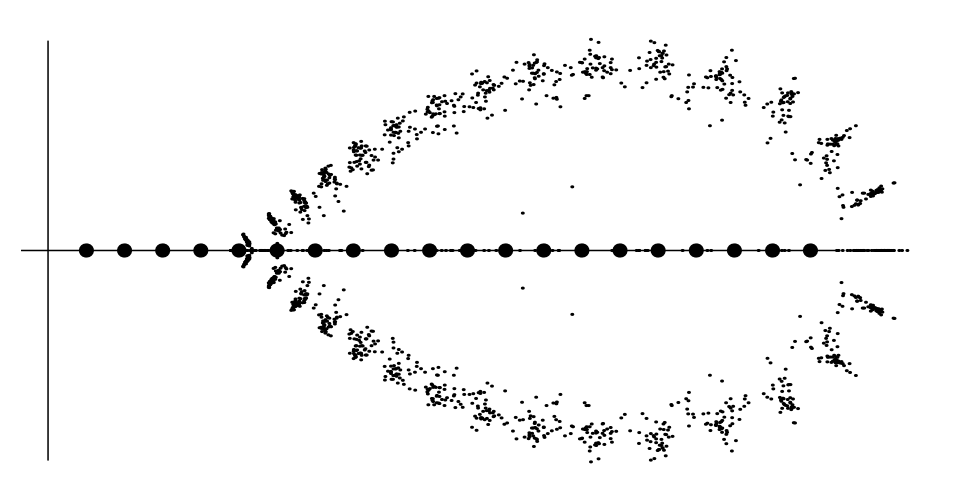
\includegraphics[width=0.5\linewidth]{assets/Screenshot 2025-04-15 at 00.21.49.png}
    \caption{Wilkinson's example 中 roots 的 perturbation, by $\tilde{a}_k=a_k\left(1+10^{-10} r_k\right)$}
    \label{fig:enter-label}
\end{figure}



\subsection{example: matrix 乘 vector}
这个 example 分为三部分: \\
For problem $Ax = b$:
\begin{enumerate}
    \item Fixing $A$, $x\mapsto b$
    \item Fixing $A$, inverse problem: $b \mapsto x$
    \item fixing $b$, $A\mapsto x$
\end{enumerate}
\begin{example}
    Matrix-vector multiplication: $Ax = b$ (fixing $A$)
$$
\begin{aligned}
&\kappa_{\mathrm{fwd}}(x)=\sup _{\delta x}\left(\frac{\|A(x+\delta x)-A x\|}{\|A x\|} / \frac{\|\delta x\|}{\|x\|}\right)=\sup _{\delta x} \frac{\|A \delta x\|}{\|\delta x\|} / \frac{\|A x\|}{\|x\|}\\
\end{aligned}
$$  即:\[
\kappa_{\mathrm{fwd}}(x)=\|A\| \frac{\|x\|}{\|A x\|}
\]
Note: 对于任意非零 $x$ , 都有
$$
\|A x\| \geq \frac{1}{\left\|A^{\dagger}\right\|} \cdot\|x\| \quad \Longrightarrow \quad \frac{\|x\|}{\|A x\|} \leq\|A^{\dagger}\|
$$所以 $$
\kappa_{\mathrm{fwd}}(x)=\|A\| \cdot \frac{\|x\|}{\|A x\|} \leq\|A\| \|A^{\dagger}\|
$$
\textbf{(2) Inverse problem: given $b$ 求 $x$, 即 $x = A^{-1} b$, 也有同样的 condition number bound (这显然，因为对称):} $$
\kappa_{\mathrm{inverse}}(b)=\left\|A^{\dagger}\right\| \frac{\|b\|}{\|x\|} \leq \|A\| \|A^{\dagger}\|
$$ 因而我们把 $\|A\| \|A^{-1}\| $ 称为 \textbf{一个 matrix 的 condition number.}
\begin{definition}{condition number of a matrix}
我们定义 condition number of a matrix: \[
    \kappa(A) := \|A\| \|A^{\dagger}\|
    \]
Notice: 如果 $\| \cdot \| : = \|\cdot \|_2$, 那么 for $A \in \mathbb{C}^{m\times n}$, we have: \[
\| A \|_2 = \sigma_1,\quad \| A ^{\dagger} \|_2 = 1/\sigma_r
\]where\textbf{ $\sigma_r$ 是最小的非零的 singular value.}
\end{definition}
对于 $\| \cdot \| : = \|\cdot \|_2$, \[
 \kappa(A) = \frac{\sigma_1}{\sigma_r}
\]即 image of the unit sphere 作为 hyperrellipse 的 eccentricity.
\end{example}
\begin{remark}
    我们已经知道了, 对于 $Ax = b$ ($A\in \mathbb{C}^{m\times n}$): 不论是 forward problem  $x\mapsto b$ 还是 inverse problem $b \mapsto x$, 都有\[
    \kappa \leq \kappa(A)
    \]
那么等号在什么时候取到呢?    我们以 forward problem 为例: 取 $A$ 的 SVD: $A=U \Sigma V^*$, where 
    \begin{itemize}
        \item $U \in \mathbb{C}^{m \times m}, V \in \mathbb{C}^{n \times n}$ unitary，
        \item $\Sigma=\operatorname{diag}\left(\sigma_1, \ldots, \sigma_r, 0, \ldots, 0\right) \in \mathbb{R}^{m \times n}, r=\operatorname{rank}(A)$ 
        \item  $\sigma_1 \geq \sigma_2 \geq \cdots \geq \sigma_r>0$
    \end{itemize}
我们令 $x=V z$ ，因为 $V$ unitary 不改变范数，
$$
A x=U \Sigma V^* V z=U \Sigma z \Rightarrow\|A x\|=\|\Sigma z\|, \quad\|x\|=\|z\|
$$
所以 $$
\frac{\|x\|}{\|A x\|}=\frac{\|z\|}{\|\Sigma z\|}=\frac{\left(\sum_{i=1}^n\left|z_i\right|^2\right)^{1 / 2}}{\left(\sum_{i=1}^r \sigma_i^2\left|z_i\right|^2\right)^{1 / 2}}
$$
这个最大值就是: $$
\max _{z \neq 0} \frac{\|z\|}{\|\Sigma z\|}=\max _{z \neq 0} \frac{1}{\left(\sum_{i=1}^r \sigma_i^2 \cdot \frac{\left|z_i\right|^2}{\|z\|^2}\right)^{1 / 2}}
$$
这在 $\left|z_i\right|=1$ 只有一个非零坐标, 且对应于最小非零奇异值 $\sigma_r$ 时最大. 所以最大值是 $1 / \sigma_r=\left\|A^{\dagger}\right\|$ 。因此：
$$
\frac{\|x\|}{\|A x\|}=\left\|A^{\dagger}\right\| \quad \Longleftrightarrow \quad x \in \operatorname{span}\left(v_r\right)
$$ 即, \textbf{当 $x$ 是 $A$ 的 minimal nonzero singular value  $\sigma_r$ 的 right singular vector 时}, 取到 \[
\kappa_{\mathrm{fwd}}(x) = \kappa(A)
\]
同理, 对于 inverse problem, 令 $b=U y$, 有:
$$
A^{\dagger} b=V \Sigma^{\dagger} U^* U y=V \Sigma^{\dagger} y \Rightarrow\left\|A^{\dagger} b\right\|=\left\|\Sigma^{\dagger} y\right\|, \quad\|b\|=\|y\|
$$
其中 $\Sigma^{\dagger}=\operatorname{diag}\left(1 / \sigma_1, \ldots, 1 / \sigma_r, 0, \ldots, 0\right)$. 所以： $$
\frac{\|b\|}{\left\|A^{\dagger} b\right\|}=\frac{\|y\|}{\left\|\Sigma^{\dagger} y\right\|}=\left(\frac{\sum_{i=1}^m\left|y_i\right|^2}{\sum_{i=1}^r \frac{1}{\sigma_i^2}\left|y_i\right|^2}\right)^{1 / 2}
$$最大值发生在 $y=e_1$ 对应于最大奇异值 $\sigma_1$, 此时
$$
\left\|A^{\dagger} b\right\|=\frac{1}{\sigma_1}\|b\| \Rightarrow \frac{\|b\|}{\left\|A^{\dagger} b\right\|}=\sigma_1=\|A\|
$$
因此
$$
\kappa_{\mathrm{inv}}(b)=\left\|A^{\dagger}\right\| \cdot\|A\| \quad \Longleftrightarrow \quad b \in \operatorname{span}\left(u_1\right)
$$

 即, \textbf{当 $b$ 是 $A$ 的 maximal singular value  $\sigma_1$ 的 left singular vector 时}, 取到 \[
\kappa_{\mathrm{inverse}}(b) = \kappa(A)
\]
\end{remark}
至此, 我们可以总结这个 theorem (a general version of Theorem 12.2 in textbook Ch12):
\begin{theorem}{conditioning of matrix times vector}
    For problem $Ax = b$  fixing $A$, 不论是 $x\mapsto b$ 的 forward problem 还是 $b \mapsto x$ 的 inverse problem, 都有: \[
    \kappa \leq \kappa(A): = \|A\| \|A^{\dagger}\|
    \]
    并且, 对于 forward problem, 等号当且仅当 $x$ 是 $A$ 的 minimal nonzero singular value  $\sigma_r$ 的 right singular vector 时取到; 对于 inverse problem, 等号当且仅当 $b$ 是 $A$ 的 maximal singular value  $\sigma_1$ 的 left singular vector 时取到.
\end{theorem}

现在我们来考虑: Fixing $b$, 求 $A \mapsto x$ 的问题.\\
我们有: $$
(A+\delta A)(x+\delta x)=b
$$
我们知道 $A x=b$, 并且可以 drop the doubly infinitesimal term $(\delta A)(\delta x)$, 从而得到$$(\delta A) x+A(\delta x)=0$$即 \[
\delta x=-A^{\dagger}(\delta A) x
\]
By matrix norm 小于等于拆分后 norms 的乘积的定理, 我们于是有: \[
\|\delta x\| \leq\left\|A^{\dagger}\right\|\|\delta A\|\|x\|
\]
即
$$
\frac{\|\delta x\|}{\|x\|} / \frac{\|\delta A\|}{\|A\|} \leq\|A^{\dagger}\|\|A\|=\kappa(A)
$$
于是我们得到 \[
\kappa_{A\mapsto x} \leq \kappa(A)
\]
神奇地发现, 它也被 $\kappa(A)$ bound.\\
并且, equality in this bound will hold whenever $\delta A$ is such that
$$
\left\|A^{\dagger}(\delta A) x\right\|=\left\|A^{\dagger}\right\|\|\delta A\|\|x\|
$$
而, 我们可以发现对于任意 $A,b$, 这个 $\delta A$ 一定存在, 即等号一定可以取到. 这是因为 operator norm 与其 dual norm 的等价性:$$
L: \delta A \mapsto A^{\dagger}(\delta A) x
$$
是一个从 $\mathbb{C}^{m \times n} \rightarrow \mathbb{C}^n$ 的线性算子, 它的 operator norm 是:
$$
\|L\|=\sup _{\delta A \neq 0} \frac{\left\|A^{\dagger}(\delta A) x\right\|}{\|\delta A\|}
$$
我们可以证明这个 supremum 可以达到. 选择
$$
\delta A=u v^*
$$
其中 $u \in \mathbb{C}^m$ 是使得 $\left\|A^{\dagger} u\right\|=\left\|A^{\dagger}\right\|$ 的单位向量, $v=\frac{x}{\|x\|}$ 是单位方向向量. 于是: $$
(\delta A) x=\left(u v^*\right) x=u \cdot\left(v^* x\right)=u \cdot\|x\| \Rightarrow A^{\dagger}(\delta A) x=\|x\| \cdot A^{\dagger} u \Rightarrow\left\|A^{\dagger}(\delta A) x\right\|=\|x\| \cdot\left\|A^{\dagger} u\right\|=\|x\| \cdot\left\|A^{\dagger}\right\|
$$
从而我们可以得到这个结论: 
\begin{theorem}{conditioning of matrix times vector: given $b$, problem$A\mapsto x$ }
对于 $Ax = b$ fixing $b$,  考虑 problem $A\mapsto x$, 这一问题一定有 condition number:  \[
\kappa = \kappa (A)
\]
\end{theorem}


\section{float number and machine epsilon}
\subsection{float number system}
我们知道计算机处理的是离散的数值. 即, 一个 computer 的 number system 并非 $\mathbb{R}$ 而是 $\mathbb{R}$ 的一个 discrete (and finite, 但是 ideally 可以看作 infinite) subset $\mathbf{F}$, 称之为 float number system.\\
这个 $\mathbf{F}$ 由这两个参数决定决定: 
\begin{itemize}
    \item base integer $\beta$
    \item precision integer $t$
\end{itemize}
(通常 $\beta =2$ 即 二进制, 而 $t = 24,53$ for IEEE single/double precision.)\\
precision 决定了这个系统的对数字表示的相对精度 (即即将定义的 machine epsilon); biased exponent 决定了这个系统能够表示的数的范围的上下限.
从而,  \[
F = \{0 \}\cup \{\pm (\frac{m}{\beta^t})  \beta^e : m\in [1,\beta^t-1] \text{ int}, e \text{ int}\}
\]
这里的 \(\pm \frac{m}{\beta^t} \)称为 \textbf{mantissa} of $x$; $e$ 称为 \textbf{exponent}.\\
现实中,  $e$ 也有范围, 取决于计算机位数和架构. 比如说 ieee 双精度 float: 这里 $E$ 的范围是 $0\sim 2047$, 因而 \textbf{$e = E - 1023$ 的范围是 $-1023\sim 1024$}.
\begin{figure}
    \centering
    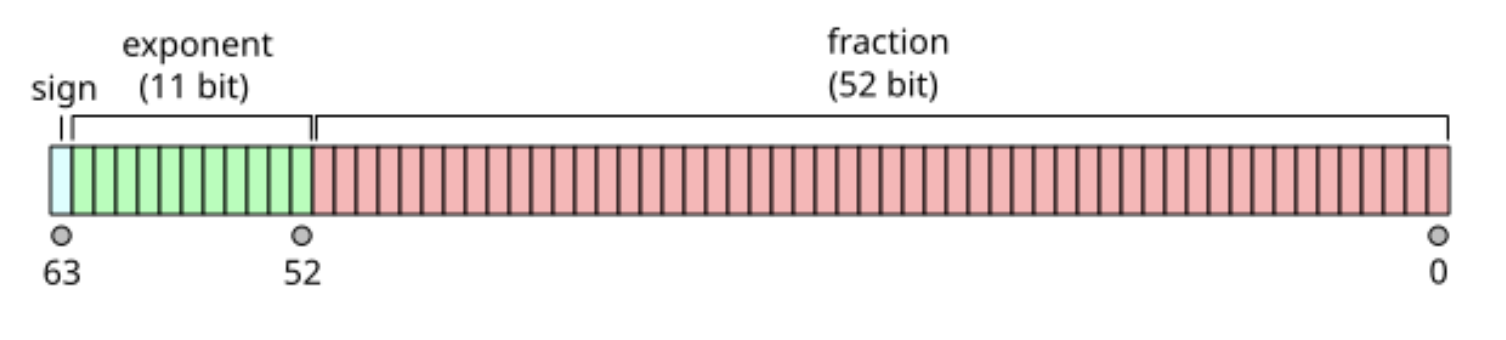
\includegraphics[width=0.5\linewidth]{assets/Screenshot 2025-04-15 at 10.56.30.png}
    \caption{IEEE}
    \label{fig:enter-label}
\end{figure}
IEEE double precision:
$$
x = (-1)^{\operatorname{sign}}\left(1 . b_{51} b_{50} \ldots b_0\right)_2 \times 2^{E-1023}
$$
因而更加现实的 system $\mathbf{F}$ 和我们这里的理论 model $\mathbf{F}$ 有这些差别:
\begin{enumerate}
    \item 还要包括一个额外的参数: exponent offset $s$, 控制 $e$ bounded by some $e_{\min}$ 和  $e_{\max}$.
    \item 现实的 ieee standard 和我们的 ideal 模型 $\mathbf{F}$ 不同的点, 不仅是 $e$ bounded 具有 $e_{\min}$ 和  $e_{\max}$, 还有: 它的每个数其实是  \[ \pm (1+\frac{m}{\beta^t})\beta^e\] 而不是 \(\pm (\frac{m}{\beta^t})\beta^e\). 前面的 $1$ 称为 leading bit. 这是因为在 规格化二进制浮点数系统中, 所有非零数的尾数都可以唯一表示成以 $1.$ 开头的形式. 因为这个 $1.$  总是存在, 可以省略它来节省空间.
    \item 考虑更多的 symbols, 例如: $$
\begin{array}{|l|l|}
\hline \text { Symbol } & \text { Meaning } \\
\hline+0 & \text { Postitive underflow; between } 0 \text { and the smallest positive representable float } \\
\hline-0 & \text { Negative underflow } \\
\hline+\infty & \text { Positive overflow; bigger than biggest representable float. E.g., } 1 / 0=1 /(+0) \\
\hline-\infty & \text { Negative overflow } \\
\hline \text { NaN } & \text { Not-a-Number, e.g., 0/0. } \\
\hline
\end{array}
$$ Note: $0$ 也是一个 symbol. 并且, 现实的 system 里, 还要区分正负方向上的 underflow 得到的 $0$.
\end{enumerate}




\begin{definition}{machine epsilon}
对于一个 discrete number system $\mathbf{F}$ with precision $t$ 和 base $\beta$,  我们定义: \[
    \epsilon_{machine}  : = \frac{1}{2} \beta^{1-t}
    \]
\end{definition}
为什么要这样定义: 因为这两点:
\begin{proposition}
    对于任意的 $x\in \mathbb{R}$ that is within machine 的表示范围, 都存在一个 $\epsilon$ s.t. $|\epsilon| < \epsilon_{machine}$ 使得 \[
    fl(x) = x(1+ \epsilon)
    \]
\end{proposition}
这一点是显然的. 任意的大小不能过大的实数, 都可以在 machine epsilon 的误差内被 float number 表示.\\
更加好的是:
\begin{theorem}{Fundamental Axion of Floating Point Arithmetic}
  对于一个 discrete number system $\mathbf{F}$, 对于任意的 $x,y\in \mathbf{F}$, 都存在一个 error $\epsilon$ s.t. \[
  |\epsilon| \leq \epsilon_{machine}
  \]such that:  $$
x *_{fl} y=(x *_{\mathbb{R}} y)(1+\epsilon)
$$
for 任意的 $* := +,-,\times ,\div$.\\
(Exclusion: relative error 并不包括 $x-x$ 时出现的 cancellation error, 以及其他的 overflow, underflow! 这些是\textbf{ symbolic hacks}, 例如 perturbing $0$ to $0.1$ gives relative error $\frac{0.1-0}{0}=+\infty$; 并且需要注意的是, relative errors are only useful when small, well below $100 \%$.)
\end{theorem}
即: 任意基本运算的相对于自身的误差, 都被 bound 在 $\epsilon_{machine}$ 之内.\\
为什么是相对误差而不是绝对误差? 因为我们能表示的有效数字位数是固定的. 越大的数, 其小数点后的有效数字就越小. 从而, 绝对误差就越大. 但是相对误差仅和 $t$ 和 base $\beta$ 有关.\\
(Note: On a computer in which intermediate quantities are \textbf{truncated rather than rounded}, Fundamental Axion of Floating Point Arithmetic hold with\textbf{ $\epsilon_{\text {machine }}$ replaced by $2 \epsilon_{\text {machine }}$}.)\\

\begin{remark}
之所以 Float number 的讨论是重要的, 因为它是计算机用来近似表示一个实数的方法, 而所有的数值计算都要经由此为媒介. 需要注意的是:\textbf{ ultimate access to numbers is via +,−,⋆,÷, 复杂度和误差最终由基本运算衡量.}\\

对于 losing 1 bit  的 round off error 等问题, 我们并不在意; 但是, 当大量计算 iteratively 堆叠时, \textbf{一些 first algorithms for many problems might lose half the bits. } 这是一个很大的数量: 例如 Classical Gram 
Schmidt 会失去 half the digits, 相比 modified Gram-Schmidt 而言. 例如, accurate bits 从 52 变为 26.\\

因而, 基于 float number (via machine epsilon) 对一个 algorithm 的 stability 进行分析是重要的. 接下来我们将讲解 stability of an algorithm 这个概念.
\end{remark}





\section{stability}
Review: 一个 Problem (in our def) 是一个 function $f:X \to Y$, $X,Y$ 都是 NVS.\\
而我们现在定义什么是一个 algorithm:
\subsection{def: algorithm, stability, accuracy}
\begin{definition}{algorithm}
    一个 algorithm for a problem $f:X\to Y$ 是另一个函数 $\tilde{f}:X \to Y$
\end{definition}
定义上就是这么简单.\\
\textbf{注意: 我们这里的 algorithm 是一个比较 restricted 的定义. Specially, 它并不考虑 randomized algorithms.}
\begin{example}
    Randomized rounding: \\
    把 $7.3$ round to: 8, with a prob of $0.3$;  $7$, with a prob of $0.7$.\\
    我们把 round 得到的结果标记为 $X$, 那么它则是一个 random variable. 并且, 它是一个 unbiased random variable, 即: \[
    \mathbb{E}[X] = 7.3
    \]
    这个 rounding 是一个 algorithm, 但是不包含在我们这里的定义里. 因为原问题是 $\mathbb{R}\to \mathbb{N}$ 的, 而这个问题则是 maps to random variables (我们知道一个 random variable 是一个函数, 这是一个 function space) 的. 因而它并不是我们定义的算法.\\
    因而我们的定义其实是 restricted 的. 我们这里只考虑 determinstic 的 algorithm.\\     
\end{example}



\begin{definition}{accuracy of an algorithm}
给定一个 problem $f$ 和一个对应的 algorithm $\tilde{f}$, 我们定义 $\tilde{f}$ 的 relative error 为$$
\frac{\|\tilde{f}(x)-f(x)\|}{\|f(x)\|}
$$
  即: algorithm 给出的答案和正确答案的相对 difference.\\
如果对于每个 $x\in X$ 都有: $$
\frac{\|\tilde{f}(x)-f(x)\|}{\|f(x)\|}=O\left(\epsilon_{\text {machine }}\right)
$$
即 relative error is on the order of machine epsilon, 那么我们称这个 algorithm 是 accurate 的.
\end{definition}
Problem: 对于一个 well-conditioned 的问题, 我们自然地想要一个足够 accurate 的 algorithm; 但是对于 ill-conditioned 的问题, 要求给出一个足够 accurate 的 algorithm 是很困难的事情, 因为 perturbations on ill-conditioned inputs 使得它给出准确结果的难度很大.\\
因而, generally, 我们应该放低要求.
\begin{definition}{stability of an algorithm}
    给定一个 problem $f$ 和一个对应的 algorithm $\tilde{f}$, 如果对于每个 $x \in X$ 都存在一个 $\tilde{x} \in X$, 其满足$$
\frac{\|\tilde{x}-x\|}{\|x\|}=O\left(\epsilon_{\text {machine }}\right)
$$能够使得  $$
\frac{\|\tilde{f}(x)-f(\tilde{x})\|}{\|f(\tilde{x})\|}=O\left(\epsilon_{\text {machine }}\right)
$$那么则称, 这个 algorithm $\tilde{f}$ 是 statble 的.
\end{definition}
\begin{remark}
  显然, stable 是比 accurate 稍微宽松的要求. 它的要求是: \textbf{这个 algorithm gives nearly the right answer to nearly the right question}. 比起 accurate, 它放宽在于: 不需要 solve exactly the same question, 只需要 solve 一个很相近的 question 就可以了.\\
  
为什么要这样要求? 因为一个计算机很大的问题是: 我们的 input 和理论上的 input 还是不一样的. 比如, 我们要输入一个 $x = \frac{2}{3}$, 这是一个无限循环的小数, 而计算机只能输入有限位数的小数来近似. 因而关于它的计算问题, 从输入起就有了误差. 这个误差可能很小, 但是一旦遇到 ill-conditioned 的问题, 在 condition 比较差的地方 (比如说某个问题在 $0$ 处, $\kappa(x) \to \infty$), 那么这个 input 的小误差很可能导致很大的 Output 不同.\\

从而, 我们需要对 input 放宽, 尽可能去容忍类似于 round up 这样的问题. \\

这个时候我有一个问题: stable 这个概念, 相比于 accurate, 是为了迁就 ill-conditioned 的问题, 只要保证我们的算法给出的结果一定是原问题周围某个相似的问题的数值解就可以了. 但是如果这个 problem 是 ill-conditioned, 那么原问题的解可能和它周围的其他问题的解差别非常大. 一个 stable 但不 accuratae 的 algorithm, 意思就是: 在某些 ill-conditioned 的 input 上, 给出的解和我们想要的原问题的解差别非常大, 那这个算法还能成为好吗?\\

这就是数值分析的核心哲学问题之一. stability 已经是一个足够的条件, 因为你并不能要求算法给你“一个问题本身都无法承诺”的东西. Stable algorithm 是对现实的诚实反应, 承认输入的不可避免误差, 并保证: 你得到的结果是"某个微小扰动问题"的真实答案. 它告诉你: \textbf{在你所能拥有的误差范围内, 这就是最合理的答案了. 稳定性 = 不人为放大错误.}\\ 
之所以我们只要求算法的稳定性, 就是因为: \textbf{如果非要要求准确性, 那么很多优秀的 algorithm 可能会因为仅仅几个 problem 本身就 ill-condtioned 的点上的大误差, 被判为 inaccurate. }  
\end{remark}

还有一个比 stable 更强的定义
\begin{definition}{backward stability}
    给定一个 problem $f$ 和一个对应的 algorithm $\tilde{f}$, 如果对于每个 $x \in X$ 都存在一个 $\tilde{x} \in X$, 其满足$$
\frac{\|\tilde{x}-x\|}{\|x\|}=O\left(\epsilon_{\text {machine }}\right)
$$能够使得 $\tilde{f}(x)= f(\tilde{x})$ 那么则称, 这个 algorithm $\tilde{f}$ 是backward stable 的.
\end{definition}
backward stable 的要求是: 这个 algorithm gives exactly the right answer to nearly the right question. \textbf{它蕴含的信息是: 对于这个算法 $\tilde{f}$, 任意的 output perturbation 其实都等同于某些 input perturbation. (从而可以被 input perturbation 给完全控制.)}\\
backward stable 和 accurate 是 dual 的: accurate 要求的是这个 algorithm gives nearly the right answer to the right question.\\
\begin{remark}
这些定义里面的 $O\left(\epsilon_{\text {machine }}\right)$ 是 across all $x$ 的, 即\textbf{存在一个 uniform bound $C\epsilon_{\text{machine}}$ among all $x\in X$, 使得这些误差值 bounded by it.}
\begin{example}
我们用一个例子来阐明 "$O\left(\epsilon_{\text {machine }}\right)$":\\
problem: 给定 $b$, solve system $Ax = b$ for $A \mapsto x$. 假设我们有一个 algorithm $\tilde{f}: A \mapsto x$ 是 \textbf{stable} 的, 那么它满足: 对于给定的 $n,m$, \textbf{存在 uniform bound $C_1,C_2$} 使得对于任意的 $A \in \mathbb{C}^{n\times m}$, 都具有 \textbf{nearly the same question $\tilde{A}$},  使得 algorithm \textbf{$\tilde{f}$ 给出的 answer $\tilde{f}(A)$ 几乎就是这个近似问题 $\tilde{A}$ 的正确解 $f(\tilde{A})$.}\\
Formally: 对于任意的 $A \in \mathbb{C}^{n\times m}$, 都存在  $\tilde{A} \in \mathbb{C}^{n\times m}$ s.t. \[
\frac{\|\tilde{A}-A\|}{\|A\|}\leq C_1 \epsilon_{\text {machine }}
\]使得 \[
\frac{\| \tilde{f}(A) - f(\tilde{A})\| }{\| f(\tilde{A}) \|}  \leq C_2 \epsilon_{\text{machine}}
\]
这个 $C_1,C_2$ 是和 input 进入的 $A$ 无关的, 它被 problem 的参数固定 (here: $n,m$). For example, $C_1 = 10,C_2 = 100$.
\end{example}
\end{remark}
\begin{remark}
    对于 finite dimensional NVS 而言, 我们不需要关注使用的是哪个 norm, 因为我们知道,  finite dimensional NVS 上所有 norms 都是 topologically equiv 的. 这个等价在这里对 asympototic bound 的讨论中很有用, 因为  topologically equiv 即: 对于任意两个 norms $\|\cdot\|_a,\|\cdot\|_b $, 都存在 $C_1, C_2$ 使得对于任何元素 $x$ 都有 \[
C_1   \| x\|_a \leq   \| x\|_b \leq C_2  \| x\|_a
    \]
    因而,   对于 finite dimensional NVS 而言, 如果任意一个 norm 满足$$
\| x\|=O\left(\epsilon_{\text {machine }}\right)
$$那么任意的 norm 都满足这一点.
\end{remark}


\subsection{example: floating point arithmetic}
\begin{example}
    当然, 四种 floating point arithmetic 是有 backward statble 的算法的.\\
我们以两数相减 from $f:\mathbb{C}^2 \to \mathbb{C}$ 为例: 我们 canonical 的算法就是把这两个数 round 为 float, 然后进行 float 的减法.
$$
\tilde{f}\left(x_1, x_2\right)=\mathrm{fl}\left(x_1\right) \ominus \mathrm{fl}\left(x_2\right) .
$$
其中, 
$$
\mathrm{fl}\left(x_1\right)=x_1\left(1+\epsilon_1\right), \quad \mathrm{fl}\left(x_2\right)=x_2\left(1+\epsilon_2\right)
$$
where by def, $|\epsilon_1|,|\epsilon_2| < \epsilon_{\text{machine}}$.\\
并且我们知道, float 减法的 error 也是 within machine epsilon 的: $$
\mathrm{fl}\left(x_1\right) \ominus \mathrm{fl}\left(x_2\right)=\left(\mathrm{fl}\left(x_1\right)-\mathrm{fl}\left(x_2\right)\right)\left(1+\epsilon_3\right)
$$
从而$$
\begin{aligned}
\mathrm{fl}\left(x_1\right) \ominus \mathrm{fl}\left(x_2\right) & =\left[x_1\left(1+\epsilon_1\right)-x_2\left(1+\epsilon_2\right)\right]\left(1+\epsilon_3\right) \\
& =x_1\left(1+\epsilon_1\right)\left(1+\epsilon_3\right)-x_2\left(1+\epsilon_2\right)\left(1+\epsilon_3\right) \\
& =x_1\left(1+\epsilon_4\right)-x_2\left(1+\epsilon_5\right)
\end{aligned}
$$
where $$
\left|\epsilon_4\right|,\left|\epsilon_5\right| \leq 2 \epsilon_{\text {machine }}+O\left(\epsilon_{\text {machine }}^2\right) = O(\epsilon_\text {machine})
$$

我们把 \[
\hat{x_1}: = x_1\left(1+\epsilon_4\right), \quad \hat{x_2} :=x_2\left(1+\epsilon_5\right)
\]
从而, 这个 canonical algorithm 计算出的是: \[
\tilde{f} (x_1, x_2) = f (\hat{x_1},\hat{x_2})
\]where for all  $(x_1, x_2) $, 它对应的这个 $ (\hat{x_1},\hat{x_2})$ 和它在 $\mathbb{C}^2$ 中的 relative distance, within any norm 都是 $O(\epsilon_\text {machine})$ 的.
\end{example}
\begin{remark}
值得提的是: 两个数相加的问题 $\mathbb{C}^2 \to \mathbb{C}$ 的 canonial algorithm 是 backward stable 的, 而一个数加一个固定的常数: $\mathbb{C}\to \mathbb{C}$ 的 canonial algorithm 却不是 backward stable 的.
\end{remark}


\subsection{example: inner/outer product }
For inner product: problem is $f: \mathbb{C}^m\times \mathbb{C}^m \to \mathbb{R}$,  given vectors $x, y \in \mathbb{C}^m$, wish to compute the inner product $\alpha=x^* y$.\\
显然, canonical algorithm: compute the pairwise products $\bar{x}_i y_i$ with $\otimes$ and add them with $\oplus$ to obtain a computed result $\tilde{\alpha}$. 
这个算法是 \textbf{backward stable} 的.\\
但是, for outer product: problem is $f:  \mathbb{C}^m \times  \mathbb{C}^n \to  \mathbb{C}^{m\times n}$ .\\
我们想要计算 $A=x y^*$, for vectors $x \in \mathbb{C}^m, y \in \mathbb{C}^n$. \\
Canonical algorithm: compute the $m n$ products $x_i \bar{y}_j$ with $\otimes$ and collect them into a matrix $\tilde{A}$. \\
它是 stable 的, 但却不是 backward stable 的. 因为直观而言: 我们 每个 entry 的计算有不同的乘法误差, 导致:  $\tilde{A}$ will 不太可能 have rank exactly 1, 因而无法真的被写作 written in the form $(x+\delta x)(y+\delta y)^*$. \\
\begin{remark}
对于 solution space $Y$ 的 dimension 比 problem space $X$ 更加大的问题 (以及 problem space 是多个输入, 其中每个输入的 space 的 dimension 比 solution space 的要小), 很少会有 backward stability.
\end{remark}


\subsection{theorem: what backward stabililty implies about the accuracy}
\begin{theorem} Suppose a backward stable algorithm is applied to solve a problem $f: X \rightarrow Y$ with condition number $\kappa$, 那么 relative errors:
$$
\frac{\|\tilde{f}(x)-f(x)\|}{\|f(x)\|}=O\left(\kappa(x) \epsilon_{\text {machine }}\right) 
$$
(notice: 这说明如果 $\kappa$ of this problem bounded, 那么 backward stable algorithm 一定是 accurate 的)
\end{theorem}
\begin{proof}
By backward stability, we have $\tilde{f}(x)=f(\tilde{x})$ for some $\tilde{x} \in X$ satisfying $$
\frac{\|\tilde{x}-x\|}{\|x\|}=O\left(\epsilon_{\text {machine }}\right) 
$$
我们把 $\tilde{x}-x$ 作为 $\delta x$, 从而有: $$
\frac{\|\delta x\|}{\|x\|}=O\left(\epsilon_{\text {machine }}\right)
$$
而由于这里 $\frac{\|\delta x\|}{\|x\|}=O\left(\epsilon_{\text {machine }}\right)$ 已经是 numerically 最小的 error. 从而   By definition of $\kappa(x)$: $$
\frac{\|f(x+\delta x)-f(x)\|}{\|f(x)\|} \leq (\kappa(x) + o(1)) \cdot \frac{\|\delta x\|}{\|x\|}
$$这个不等式是因为: $f$ 的相对变化和 $x$ 的相对变化的比例, 其上极限就是 $\kappa (x)$. 从而 this implies
$$
\frac{\|\tilde{f}(x)-f(x)\|}{\|f(x)\|}  = \frac{\|{f}(x)-f(\tilde{x})\|}{\|f(x)\|}  = \frac{\|f(x+\delta x)-f(x)\|}{\|f(x)\|}\leq(\kappa(x) + o(1)) \cdot \frac{\|\delta x\|}{\|x\|}
$$
\end{proof}
这一 theorem 表明: backward stability + good conditioning $\implies$ accuratcy









\chapter{backward error analysis of NLA algorithms\cite{doi:10.1137/1.9780898719574.ch3}}
我们在上一个 Ch 中介绍了 conditioning 和 stability. 现在我们用它们对经典的 NLA algorithms 进行 backward error analysis.


\section{Stability of Householder Triangularization}
我们 set $R, Q$ to be random upper triangular 和 orthogonal matrices (by orthogonizing 一个 random matrix), 并 set $A : = QR$.
\begin{verbatim}
    R = triu (randn(50));
    [Q,X] = qr(randn(50));
    A = Q*R
\end{verbatim}
然后我们再对 $A$ 进行 QR 分解, via Household (Matlab 自带使用 Household), 看看 relative error: 
\begin{verbatim}
    [Q2,R2] = qr(A);
    norm (Q2 - Q);
        ans = 0.00889
    norm (R2-R) / norm(R);
        ans = 0.00071
\end{verbatim}
我们发现 $Q,R$ 的 relative error 其实很大.\\
但是, 当我们用这个 $QR$ 计算 $A$ 时:
\begin{verbatim}
    norm (A - Q2*R2) / norm(A);
        ans = 1.432e-15
\end{verbatim}
我们发现一个惊人的事实: 这个 QR 分解的 error 


$$
\begin{aligned}
& \text { Q3 }=\mathrm{Q}+1 \mathrm{e}-4 * \operatorname{randn}(50) ; \\
& \text { R3 }=\mathrm{R}+1 \mathrm{e}-4 * \operatorname{randn}(50) ; \\
& \text { norm }(\mathrm{A}-\mathrm{Q} 3 * \mathrm{R} 3) / \operatorname{norm}(\mathrm{A}) \\
& \text { ans }=0.00088
\end{aligned}
$$







\section{Stability of Back Substitution}








\section{Conditioning of Least Squares}







\section{Stability of Least Squares}




















\printbibliography
\appendix




\end{document}